\documentclass{tstextbook}

\usepackage{glossaries}
\usepackage{tikz-cd}

\providecommand{\tq}{\mid}
\providecommand{\N}{\mathbb{N}}
\providecommand{\Z}{\mathbb{Z}}
\providecommand{\Q}{\mathbb{Q}}
\providecommand{\R}{\mathbb{R}}
\providecommand{\C}{\mathbb{C}}
\providecommand{\H}{\mathcal{H}}
\providecommand{\Im}[1]{Im(#1)}
\providecommand{\Re}[1]{Re(#1)}
\providecommand{\conjugate}[1]{\bar{#1}}
\providecommand{\pescalar}[2]{\langle #1,#2 \rangle}
\providecommand{\braket}[2]{\left\langle#1\mid#2\right\rangle}
\providecommand{\bra}[1]{\left\langle#1\right\rvert}
\providecommand{\ket}[1]{\left\lvert#1\right\rangle}
\providecommand{\so}{\Rightarrow}
\providecommand*{\circled}[1]{\tikz[baseline=(char.base)]{\node[shape=circle,draw,inner sep=2pt] (char) {#1};}}
\providecommand{\by}[1]{\overset{\fbox{\tiny #1}}{=}}
\providecommand{\maps}[3]{#1:#2\longrightarrow #3}
\providecommand{\coma}{,\thinspace}
\providecommand{\pari}[2]{(#1,\thinspace #2)}
\providecommand{\cartalocal}{(\mathcal{M}^n,\thinspace p,\thinspace U,\thinspace \varphi)\textmd{ una carta local}}
\providecommand{\doscartaslocales}{(\mathcal{M}^n\coma p\coma U\coma\varphi)\textmd{ y } (\mathcal{N}^m\coma q\coma
V\coma\psi)\textmd{ dos cartas locales}}
\providecommand{\indexdots}[3]{#1=#2,\ldots,#3}
\providecommand{\define}[2]{\textbf{#1}\label{def:#2}}
\providecommand{\avg}[1]{\left\langle#1\right\rangle}
\providecommand{\abs}[1]{\lvert#1\rvert}
\providecommand{\nor}[1]{\lVert#1\rVert}
\providecommand{\operatoravg}[3]{\left\langle#1|#2|#3\right\rangle}
\providecommand{\cinfinity}[1]{\mathscr{C}^\infty(#1)}
\providecommand{\mapsdef}[5]{ #1:\ #2 & \longrightarrow #3 \\ #4 & \longmapsto #5}
\providecommand{\glossarydef}[3]{\newglossaryentry{#1}{name={#2},description={#3}}\gls{#1}}
\providecommand{\lie}[2]{[#1\coma #2]}
\providecommand{\metrica}{\mathsf{g}}
\providecommand{\vec}[1]{\overrightarrow{#1}}
\newcommand{\set}[1]{\left\{#1\right\}}
\newcommand{\where}{\mathrel{}\middle|\mathrel{}}
\renewcommand*{\hbar}{{\mkern-1mu\mathchar'26\mkern-8mu\mathrm{h}}}
\renewcommand{\c}{\mathrm{c}}
\newcommand{\h}{\mathrm{h}}
\newcommand{\amplitud}{\mathrm{A}}
\newcommand{\longonda}{\lambda}
\newcommand{\frecuencia}{\nu}
\newcommand{\fase}{\alpha}
\newcommand{\frecuenciaangular}{\omega}
\newcommand{\longondaangular}{\mathrm{K}}
\newcommand{\periodo}{\mathrm{T}}
\newcommand{\energia}{\mathrm{E}}
\newcommand{\fuconda}{\Psi}
% Box color
\newcommand{\colorequation}[3]{\tcboxmath[on line,
    fonttitle=\small\sffamily,
    colbacktitle=#2!10!white,coltitle=#2!50!black,
    title=\small{#1},
    arc=0pt,outer arc=0pt,
    colback=#2!10!white,colframe=#2!50!black,
    boxsep=1pt,left=1pt,right=1pt,top=1pt,bottom=1pt,
    boxrule=0pt]{#3}}

% From mandi package
\newcommand{\usk}{\cdot}
\newcommand{\kilogram}{\mathrm{kg}}
\newcommand{\meter}{\mathrm{m}}
\newcommand{\second}{\mathrm{s}}
\newcommand{\inverse}{^{-1}}           % postfix -1
\newcommand{\tothetwo}{^2}             % postfix  2
\newcommand{\tothethree}{^3}           % postfix  3
\newcommand{\tothefour}{^4}            % postfix  4
\newcommand{\tento}[1]{10^{#1}}
\newcommand{\xtento}[1]{\times\tento{#1}}
%Constantes
\providecommand{\speedoflightsymbol}{\c}
\providecommand{\speedoflightvalue}{2.99792458\times10^{8}}
\providecommand{\speedoflightounits}{\meter\usk\second\inverse}
\providecommand{\plancksymbol}{\h}
\providecommand{\planckvalue}{6.62607015\times10^{-34}}
\providecommand{\planckunits}{\kilogram\usk\meter\tothetwo\usk\second\inverse}
\providecommand{\planckbarsymbol}{\hbar}
\providecommand{\planckbarvalue}{1.054571817\times10^{-34}}
\providecommand{\planckbarunits}{\kilogram\usk\meter\tothetwo\usk\second\inverse}
%Unidades
\providecommand{\mass}[1]{#1\ \kilogram}
\providecommand{\espacio}[1]{#1\ \meter}
\providecommand{\velocity}[1]{#1\ \meter\usk\second\inverse}
\providecommand{\momento}[1]{#1\ \kilogram\usk\meter\usk\second\inverse}

\newcommand\ct[1]{\text{\rmfamily\upshape #1}}
\makeglossaries
\overfullrule=1mm
\begin{document}

    \tsbook{Apuntes en mecánica cuántica}
    {Francisco Costa}
    {podxboq}
    {2021}
    {xxxxx}{xxx--xx--xxxx--xx--x}{0.1}
    {Autor independiente}
    {Murcia}

    %\printglossaries

    \section{La onda}\label{sec:la-onda}

Para la física, una onda consiste en la propagación de una perturbación de energía sin transporte de materia.

La magnitud física cuya perturbación se propaga se expresa como una función tanto de la posición como del tiempo
$\psi(\vec{r},t)$.

Matemáticamente se dice que dicha función es una onda si verifica la ecuación de ondas:
\begin{equation}
    \label{eq:ecuacion-onda}
    \nabla^2\psi(\vec {r},t)=\frac {1}{v^2}\frac{\partial^2\psi}{\partial t^2}(\vec {r},t)
\end{equation}
donde $v$ es la velocidad de propagación de la perturbación.

\subsection{Elementos de una onda}\label{subsec:elementos-de-una-onda}

\begin{description}
    \item[Cresta.] El punto de máxima separación con respecto de su posición de reposo.
    \item[Valle.] El punto de máxima elongación de la onda, en sentido opuesto a la cresta.
    \item[Amplitud ($A$).] La distancia vertical desde una cresta hasta el punto de equilibrio.
    \item[Longitud de onda ($\lambda$).] La distancia entre dos crestas consecutivas.
    \item[Número de onda angular ($k$)]. La inversa de la longitud de onda en radianes.
    \item[Periodo ($T$).] El tiempo empleado en completar una longitud de onda.
    \item[Frecuencia ($\nu$).] El número de periodos por unidad de tiempo.
    \item[Frecuencia angular ($\omega$).] La frecuencia en radianes por segundo.
    \item[Fase ($\alpha$).] El mínimo valor que hace cíclica la posición.
    \item[Velocidad de fase ($v_f$).] La velocidad a la que se propaga el movimiento ondulatorio.
    \item[Velocidad de grupo ($v_g$).] La velocidad a la que se propaga las variaciones de la amplitud.
\end{description}

Aplicando las definiciones anteriores, tenemos: $k=\frac{2\pi}{\lambda}$, $\nu=\frac{1}{T}$,
$v_f=\frac{\lambda}{T}=\nu\lambda$ y $\omega=2\pi\nu$.

\begin{figure}[htbp]
    \centering
    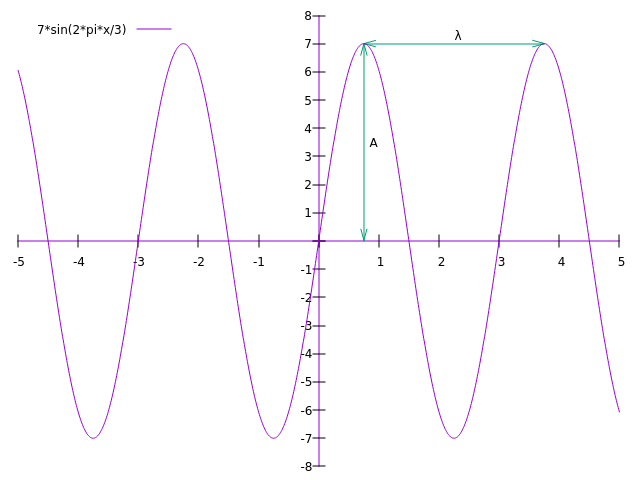
\includegraphics[width=0.6\textwidth]{sin.png}
    \caption{Elementos de una onda}
    \label{fig:elementos-onda}
\end{figure}

\subsection{Soluciones a la ecuación de onda}\label{subsec:soluciones-a-la-ecuación-de-onda}
La solución más sencilla a la ecuación de ondas es considerar una onda plana que se desplaza longitudinalmente en la dirección de la onda, donde si situamos el sistema de referencia en un punto de equilibrio tenemos la solución:
\begin{equation}
    \label{eq:solucion-ecuacion-ondas-simple}
    \psi(x,t)=A\sin(\omega t-kx)
\end{equation}

Pero la luz en una onda electro-magnética y como ya apreción Maxwell, el campo magnético aporta una componente a las ecuaciones en forma de onda compleja, y en este caso, la solución más sencilla de onda electro-magnética plana que se desplaza longitudinalmente en la dirección de la onda es:
\begin{equation}
    \label{eq:solucion-ecuacion-ondas-complejas-simple}
    \psi(x,t)=Ae^{i(\omega t-kx)}
\end{equation}

\section{Dualidad onda-partícula de De Broglie}\label{sec:dualidad-onda-partícula-de-de-broglie}

Si los fotones son partículas y ondas a la vez, podemos usar el postulado de la mecánica relativista de Einstein para partículas, y a la vez, el postulado de Planck para ondas.

\begin{postulate}[Valor de la energía de las ecuaciones de Einstein]
    \label{pos:energia_einstein}
    E=mc^2=pc
\end{postulate}

\begin{postulate}[Valor de la energía de las ecuaciones de Planck]
    \label{pos:energia_planck}
    E=h\nu=\frac{hc}{\lambda}
\end{postulate}

Así pues igualando ambas energías obtenemos la relación para cada partícula entre su momento y su longitud de onda:
\begin{postulate}[Relación entre longitud de onda y momento de De Broglie]
    \label{pos:dualidad_de_broglie}
    \lambda=\frac{h}{p}
\end{postulate}

\begin{example}
    Calcular la longitud de onda de una persona de masa $8$ kg cuando anda a una velocidad de $45$ km/h.

    La persona tiene un momento de $8*45*1000/3600=1000$ Kg m/s. Así que la longitud de onda asociada es de $\lambda=\frac{6,6256*10^{-34}}{1000}=6,6256*10^{-37}$ metros.
\end{example}

\begin{note}
    La longitud de onda más pequeña que actualmente podemos observar es del orden de $10^{-20}$ metros con el \textbf{Cherenkov telescope array}.
\end{note}

\subsection{Conclusiones}
Usando la nueva relación entre longitud de onda y momento, podemos obtener las siguientes igualdades:
\begin{equation}
    \label{eq:k_debroglie}
    k=\frac{2\pi}{\lambda}\by{\ref{pos:dualidad_de_broglie}}\frac{2\pi p}{h}=\frac{p}{\hbar}
\end{equation}
\begin{equation}
    \label{eq:omega_planck}
    \omega=2\pi\nu\by{\ref{pos:energia_planck}}2\pi\frac{E}{h}=\frac{E}{\hbar}
\end{equation}
\begin{equation}
    \label{eq:omega_debroglie}
    \omega\by{\ref{eq:omega_planck}}\frac{E}{\hbar}=\frac{p^2}{2m\hbar}\by{\ref{pos:dualidad_de_broglie}}\frac{h^2}{\lambda^2 2m\hbar}=\frac{2\pi h}{\lambda^2 2m}=\frac{\hbar k^2}{2m}
\end{equation}
\begin{equation}
    \label{eq:frecuencia_debroglie}
    \nu\by{\ref{pos:energia_planck}}\frac{E}{h}=\frac{p^2}{2mh}\by{\ref{pos:dualidad_de_broglie}}\frac{h^2}{2mh\lambda^2}=\frac{h}{2m\lambda^{2}}
\end{equation}

\subsection{Solución de onda momento-energía}\label{subsec:solucion-de-onda-momento-energia}
Una consecuencia interesante de la dualidad onda-partícula de De Blogie, es poder expresar la solución de onda electro-magnética en función de su energía y su momento.

\begin{equation}
    \label{eq:ecuacion_onda_momento_energia}
    \psi(x,t)=Ae^{i(\omega t-kx)}\by{\ref{eq:omega_planck} y \ref{eq:k_debroglie}}Ae^{i(\frac{E}{\hbar} t-\frac{p}{\hbar}x)}=Ae^{i(\hbar^{-1}(E t-p x))}
\end{equation}

\subsection{Desarrollo de la ecuación de Schröndiger}\label{subsec:desarrollo-de-la-ecuación-de-schrondiger}

Partimos de la solución de onda momento-energía (\ref{eq:ecuacion_onda_momento_energia}), calculamos la derivada parcial respecto del tiempo y la segunda derivada parcial respecto del espacio dos veces y recordando que la energia es la suma de la energía cinética y energía potencial.
\begin{equation*}
    \frac{\partial\psi}{\partial x}=\frac{ip}{\hbar}\psi\text{ y }\frac{\partial^2\psi}{\partial x^2}=\frac{-p^2}{\hbar^2}\psi
\end{equation*}

\begin{equation*}
    \frac{\partial\psi}{\partial t}=\frac{-iE}{\hbar}\psi=\frac{-ip^2}{2m\hbar}\psi+\frac{-iV}{\hbar}\psi=\frac{-i\hbar}{2m}\frac{p^2}{\hbar^2}\psi+\frac{-iV}{\hbar}\psi=\frac{i\hbar}{2m}\frac{\partial^2\psi}{\partial x^2}+\frac{-iV}{\hbar}\psi\so
\end{equation*}

\begin{equation}
    \label{eq:desarrollo-3ecuacion-schrodinger}
    i\hbar\frac{\partial\psi}{\partial t}=\frac{-\hbar^2}{2m}\frac{\partial^2\psi}{\partial x^2}+V\psi
\end{equation}




    %\chapter{1}\label{ch:1}

\section{El camino a los espacios de Hilbert}
Mientras no se indique lo contrario, siempre un espacio vectorial será un $\C$-espacio vectorial.

\subsection{Espacios métricos}
\begin{definicion}
  \label{distancia}
  Sea $E$ un espacio vectorial, diremos que la aplicación $d:E \rightarrow \R$ es una \define{métrica} sobre $E$ si cumple:
  \begin{itemize}
    \item $\forall x,y \in E,\ d(x,y)=d(y,x)$.
    \item $\forall x,y,z \in E,\ d(x,z)\leq d(x, y)+d(y, z)$.
    \item $\forall x, y \in E,\ d(x,y)\geq 0 \text{ siendo } d(x,y)=0\Leftrightarrow x = y$.
  \end{itemize}
\end{definicion}

\begin{definicion}
  \label{espacio_metrico}
  Sea $E$ un espacio vectorial y $d$ una métrica sobre $E$, llamamos al par $(E, d)$ un \define{espacio métrico}.
\end{definicion}

\subsection{Espacios normados}
\begin{definicion}
  \label{norma}
  Sea $E$ un espacio vectorial, diremos que la aplicación $\nor{}:E \rightarrow \R$ es una \define{norma} sobre E si cumple:
  \begin{itemize}
    \item $\forall x \in E,\ \forall\alpha\in\C,\ \nor{\alpha x}=\abs{\alpha}\nor{x}$.
    \item $\forall x,y \in E,\ \nor{x+y}\leq\nor{x}+\nor{y}$.
    \item $\forall x \in E,\ \nor{x}\geq 0 \text{ siendo } \nor{x}=0\Leftrightarrow x = 0$.
  \end{itemize}
\end{definicion}

\begin{definicion}
  \label{espacio_normado}
  Sea $E$ un espacio vectorial y $\nor{}$ una norma sobre $E$, llamamos al par $(E, \nor{})$ un \define{espacio normado}.
\end{definicion}

Todo espacio normado $(E, \nor{})$, es un espacio métrico, definiendo la métrica para cada par de elementos, $x, y\in E$ por $d(x, y)=\nor{x-y}$. Esta métrica se denomina \define{métrica definida por la norma}.

\definicion{Sean $(E, \nor{})$ y $(E', \nor{}')$ dos espacios normados. Sea f un homomorfismo entre E y E'. Diremos que \define{f es acotado} si existe
$c\in\R^+$ tal que $\nor{f(x)}' \leq c\nor{x}\ \forall x\in E$. Diremos que c es una \define{cota de f}.}

\definicion{Sea f un homomorfismo acotado sobre dos espacios normados. Llamamos \define{norma de f} al ínfimo de las
cotas de f.}

\resultado{
Un homomorfismo sobre espacios normados es continuo si y sólo si es acotado.
}

\resultado{
Un homomorfismo sobre espacios normados es continuo si y sólo si es continuo en un elemento.
}

\ejercicio{
Sean $E$ y $F$ dos espacios normados y $C$ el espacio vectorial de los homomorfismo acotados de $E$ en $F$. Demostrar que $\forall\ T\in C$ definiendo $\nor{T}=\text{sup}_{x\in E-\{0\}}\frac{\nor{T(x)}}{\nor{x}}$ es una norma en $C$.
}

\subsection{Espacios Euclídeos}
\begin{definicion}
  \label{producto_escalar}
  Sea $E$ un espacio vectorial, diremos que la aplicación $\braket{}{}:E\times E \rightarrow \C$ es un \define{producto escalar} sobre E si cumple:
  \begin{itemize}
    \item $\forall x,y \in E,\ \braket{x}{y}=\overline{\braket{y}{x}}$.
    \item $\forall x,y,z \in E, \braket{x}{y+z}=\braket{x}{y}+\braket{x}{z}$.
    \item $\forall x,y \in E,\ \forall\alpha\in\C, \braket{x}{\alpha y}=\overline{\alpha}\braket{x}{y}$.
    \item $\forall x \in E, \braket{x}{x}\geq 0 \text{ siendo } \braket{x}{x}=0\Leftrightarrow x = 0$.
  \end{itemize}
\end{definicion}

\begin{definicion}
  \label{espacio_euclideo}
  Sea $E$ un espacio vectorial y $\braket{}{}$ un producto escalar sobre $E$, llamamos al par $(E, \braket{}{})$ un \define{espacio euclídeo}.
\end{definicion}

Todo espacio euclídeo $(E, \braket{}{})$, es un espacio normado, definiendo la norma para cada $x\in E$, por $\nor{x}=\sqrt{\braket{x}{x}}$. Esta norma se denomina \define{norma definida por el producto escalar}.

En realidad, no es necesario indicar cual es la métrica, la norma o el producto escalar usado, pues siempre sabemos cada elemento a que espacio pertenece, así pues, sólo diremos que $E$ es un espacio métrico, euclídeo o normado y siempre denotaremos por $d$ la métrica, por $\nor{}$ la norma y por $\braket{}{}$ el producto escalar.

\begin{resultado}[Riesz]
  Sean $E$ y $F$ dos espacios euclídeos y $C$ el espacio normado de los homomorfismos acotados entre $E$ y $F$. Para cada $f\in C$, existe $z_f\in E$ tal que para todo $x\in\ E$ se tiene que $f(x)=\braket{x}{z_f}$ y además $\nor{z_f}=\nor{f}$.
\end{resultado}

\begin{definicion}
  Sea $(E, \braket{}{})$ un espacio euclídeo, con $X=\{x_n\}_{n\in\N}$ un conjunto de vectores linealmente independintes. Si $x\in E$, llamamos \define{serie de Fourier de $x$ con respecto a $X$} a
  \begin{equation}
    \sum_{n\in\N}\braket{x}{x_n}x_n
  \end{equation}
\end{definicion}

\begin{resultado}
  \label{norma_suma_general}
  Sea E un espacio euclídeo, dados $f,g\in E$ y $a,b\in\C$, se tiene la siguiente igualdad:
  \begin{equation}
    \nor{af+bg}^2=\abs{a}^2\nor{f}^2+\abs{b}^2\nor{g}^2+2\Re(a\overline{b}\braket{f}{g})
  \end{equation}
\end{resultado}
\begin{proof}
  \nor{af+bg}^2=\braket{af+bg}{af+bg}=\braket{af}{af}+\braket{af}{bg}+\braket{bg}{af}+\braket{bg}{bg}=\abs{a}^2\nor{f}^2+a\overline{b}\braket{f}{g}+b\overline{a}\braket{g}{f}+\abs{b}^2\nor{g}^2=\abs{a}^2\nor{f}^2+\abs{b}^2\nor{g}^2+a\overline{b}\braket{f}{g}+\overline{a\overline{b}}\overline{\braket{f}{g}}=\abs{a}^2\nor{f}^2+\abs{b}^2\nor{g}^2+a\overline{b}\braket{f}{g}+\overline{a\overline{b}\braket{f}{g}}=\abs{a}^2\nor{f}^2+\abs{b}^2\nor{g}^2+2\Re(a\overline{b}\braket{f}{g}).
\end{proof}
\begin{resultado}
  \label{producto_escalar_real}
  Sea E un espacio euclídeo, dados $f,g\in E$ se tiene la siguiente desigualdad:
  \begin{equation}
    \Re(\braket{f}{g})\leq\frac{1}{2}(\nor{f}^2+\nor{g}^2)
  \end{equation}
\end{resultado}
\begin{proof}
  Usando el resultado \ref{norma_suma_general} para $a=1$ y $b=-1$ tenemos que $\abs{a}=1$, $\abs{b}=1$ y $a\overline{b}=-1$ y la igualdad queda
  \begin{equation*}
    \nor{f-g}^2=\nor{f}^2+\nor{g}^2+2\Re(-\braket{f}{g})
  \end{equation*}
  Como la norma de cualquier vector es mayor o igual que cero, tendremos que
  $0\leq\nor{f}^2+\nor{g}^2+2\Re(-\braket{f}{g})=\nor{f}^2+\nor{g}^2-2\Re(\braket{f}{g})\Rightarrow 2\Re(\braket{f}{g})\leq\nor{f}^2+\nor{g}^2\Rightarrow \Re(\braket{f}{g})\leq\frac{1}{2}(\nor{f}^2+\nor{g}^2)$.
\end{proof}

\begin{resultado}
  \label{exponencial_producto_interno_real}
  Sea E un espacio euclídeo, dados $f,g\in E$ se tiene la siguiente igualdad:
  \begin{equation}
    max\{\Re(e^{i\alpha}\braket{f}{g})\text{ tq }\alpha\in\C\}=\abs{\braket{f}{g}}
  \end{equation}
\end{resultado}
\begin{proof}
  Tenemos que $\braket{f}{g}=a+ib$ para algún $a,b\in\R$. Así que $e^{i\alpha}\braket{f}{g}=(\cos(\alpha)+i \sin(\alpha))(a+ib)=(a \cos(\alpha)-b \sin(\alpha)) + i(b \cos(\alpha)+a\sin(\alpha)).$

  Por tanto, la parte real es $\Re(e^{i\alpha}\braket{f}{g})=a \cos(\alpha)-b \sin(\alpha)$ para todo $\alpha\in\C$, por lo tanto la parte real está incluido en la circunferencia de radio $\sqrt{a^2+b^2}$ y el máximo de estos valores se alcanza precisamente en la frontera del círculo, es decir $\sqrt{a^2+b^2}$ que es $\abs{\braket{f}{g}}$.
\end{proof}
\begin{resultado}
  \label{norma_producto_escalar_producto_norma}
  Sea E un espacio euclídeo, dados $f,g\in E$ se tiene la siguiente desigualdad:
  \begin{equation}
    \abs{\braket{f}{g}}\leq\nor{f}\nor{g}
  \end{equation}
\end{resultado}

\begin{proof}
  Usando el resultado \ref{norma_suma_general} y fijando $\alpha\in\C$, para $a=\frac{\nor{g}}{\nor{f}}e^{i\alpha}$ y $b=-\frac{\nor{f}}{\nor{g}}$ tenemos que $\abs{a}=\frac{\nor{g}}{\nor{f}}$, $\abs{b}=\frac{\nor{f}}{\nor{g}}$ y $a\overline{b}=-e^{i\alpha}$ y la igualdad queda
  \begin{multline*}
    \nor{\frac{\nor{g}}{\nor{f}}e^{i\alpha}f-\frac{\nor{f}}{\nor{g}}g}^2=\frac{\nor{g}}{\nor{f}}\nor{f}^2+\frac{\nor{f}}{\nor{g}}\nor{g}^2+2\Re(-e^{i\alpha}\braket{f}{g})=\\
    =\nor{g}\nor{f}+\nor{f}\nor{g}-2\Re(e^{i\alpha}\braket{f}{g})=2(\nor{f}\nor{g}-\Re(e^{i\alpha}\braket{f}{g}))
  \end{multline*}
  Como la norma de cualquier vector es mayor o igual que cero, tenemos que
  $0\leq\nor{f}\nor{g}-\Re(e^{i\alpha}\braket{f}{g})\Rightarrow \Re(e^{i\alpha}\braket{f}{g})\leq\nor{f}\nor{g}$.

  Como la desigualdad anterior es válida para todo $\alpha\in\C$ y usando el resultado \ref{exponencial_producto_interno_real} tendremos que $ \abs{\braket{f}{g}}\leq\nor{f}\nor{g}$.
\end{proof}

\begin{resultado}
  Sea E un espacio euclídeo, dados $f,g\in E$ se tiene que:
  \begin{equation}
    \label{norma_producto_escalar_igual_producto_norma}
    \abs{\braket{f}{g}}=\nor{f}\nor{g}\Leftrightarrow \exists\alpha\in\C\text{ tq }f=\alpha g
  \end{equation}
\end{resultado}

\begin{proof}
  Primero vamos a considerar el caso $f=\alpha g$:
  \begin{equation*}
    \abs{\braket{f}{g}}=\abs{\braket{\alpha g}{g}}=\abs{\alpha}\nor{g}^2=\abs{\alpha}\nor{g}\nor{g}=\nor{f}\nor{g}
  \end{equation*}
  Para el caso contrario, como se comprobó en el resultado \ref{norma_producto_escalar_producto_norma}, $\braket{f}{g}$ es el valor máximo de $\Re(e^{i\alpha}\braket{f}{g})$. Como dichos valores forman un conjunto cerrado, el máximo se alcanza, es decir, existe $\beta\in\C$ tal que $\Re(e^{i\beta}\braket{f}{g})=\abs{\braket{f}{g}}$ y utilizando el resultado \ref{norma_suma_general} para $a=\frac{\nor{g}}{\nor{f}}e^{i\beta}$ y $b=-\frac{\nor{f}}{\nor{g}}$ tenemos que:
  \begin{multline*}
    \nor{\frac{\nor{g}}{\nor{f}}e^{i\beta}f-\frac{\nor{f}}{\nor{g}}g}=2(\nor{f}\nor{g}-\Re(e^{i\beta}\braket{f}{g}))=2(\nor{f}\nor{g}-\braket{f}{g})=\\
    =2(\nor{f}\nor{g}-\nor{f}\nor{g})=0
  \end{multline*}
  Si la norma es igual que cero, tenemos que
  $\frac{\nor{g}}{\nor{f}}e^{i\beta}f=\frac{\nor{f}}{\nor{g}}g\Rightarrow f=e^{-i\beta}\frac{\nor{f}^2}{\nor{g}^2}g$. Y por tanto para $\alpha=e^{-i\beta}\frac{\nor{f}^2}{\nor{g}^2}$ tenemos la igualdad buscada.
\end{proof}

\subsection{Espacios de Banach}
\begin{definicion}
  \label{espacio_banach}
  Un espacio normado es un \define{espacio de Banach} si es completo para la métrica definida por la norma.
\end{definicion}

\subsection{Espacios de Hilbert}
\begin{definicion}
  \label{espacio_hilbert}
  Un espacio euclídeo es un \define{espacio de Hilbert} si es completo para la norma inducida.
\end{definicion}

\resultado[Ortogonalización de Gram-Schmidt]{
Todo subespacio vectorial de un espacio de Hilbert admite una base ortonormal.
}
\resultado{
Sean $E$ y $F$ dos espacios de Hilbert. Para todo homomorfismo $f$ de $E$ a $F$ existe un homomorfismo $f^+$ de $F$ a $E$ tal que $\braket{f(x)}{y}=\braket{x}{f^+(y)}$.
}

\begin{definicion}
  \label{homomorfismo_adjunto}
  Sean $E$ y $F$ dos espacios de Hilbert y $f$ un homomorfismo de $E$ a $F$. Llamamos \define{homomorfismo adjunto de f} al homomorfismo $f^+$ de $F$ a $E$ tal que $\braket{f(x)}{y}=\braket{x}{f^+(y)}$.
\end{definicion}

\resultado{
Sean $f$ y $g$ homomorfismos entre espacios de Hilbert. Se cumple:
\begin{itemize}
  \item $(f^+)^+=f$.
  \item $(af)^+=\overline{a}f^+$ para todo $a\in\C$.
  \item $(fg)^+=g^+f^+$.
\end{itemize}
}

\resultado{
Sean $f$ y $g$ dos homomorfismos entre espacios de Hilbert. El producto $fg$ es hermítico si y sólo si $f$ y $g$ conmutan.
}

\definicion{
Sean $f$ y $g$ dos homomorfismos entre espacios de Hilbert. Llamamos \define{conmutador de f}
}

\resultado{
Sean $f$ y $g$ dos homomorfismos entre espacios de Hilbert.
}

\begin{definicion}
  \label{automorfismo_autoadjunto}\label{automorfismo_hermitico}
  Sean $E$ un espacio de Hilbert y $f$ un automorfismo de $E$. Diremos que \define{f es autoadjunto} o \define{hermítico} si $f = f^+$.
\end{definicion}

\begin{definicion}
  Sean $E$ y $F$ dos espacios de Hilbert y $f$ un homomorfismo de $E$ a $F$. Diremos que \define{$f$ es compacto} si para toda sucesión $(x_n)_{n\in\N}$ de $E$, la sucesión $(f(x_n))_{n\in\N}$ tiene una subsucesión convergente.
\end{definicion}

\resultado{
Todo automorfismo compacto y hermítico sobre un espacio de Hilbert tiene su norma o el opuesto de su norma como valor própio.
}

\resultado[Teorema espectral]{
Sea $E$ un espacio de Hilbert y $f$ un automorfismo hermítico y compacto. El conjunto de todos los autovectores ortonormales de $f$ es numerable.
}

\subsection{Espacios de Hilbert separable}
\begin{definicion}
  \label{espacio_hilbert_separable}
  Un espacio de Hilbert es un \define{espacio de Hilbert separable} si tiene un subconjunto denso numerable.
\end{definicion}

\resultado{
Sea $E$ un espacio de Hilbert separable y $f$ un automorfismo de $E$. Si $f$ tiene un número infinito de valores propios distintos, entonces es una cantidad numerable y ordenados de mayor a menor definen una sucesión convergente a 0.
}

\resultado{
Sea $E$ un espacio de Hilbert separable y $f$ un automorfismo hermítico y compacto. El conjunto $\{e_n\}_{n\in\N}$ de todos los vectores propios ortonormales de $f$ es una base de $E$. Ademas se tiene que para todo $x\in\ E$, $f(x)=\sum_{n\in\N}\lambda_n\braket{x}{e_n}e_n$, donde $\lambda_n$ es el valor propio asociado al vector propio $e_n$.
}

\resultado{
En un espacio de Hilbert separable, todos los conjuntos ortogonales son numerables.
}

    %\chapter{2}\label{ch:2}
\section{Matrices}

Mientras no se indique lo contrario, las matrices son cuadradas, de dimensión $n$ y sobre el cuerpo de los números complejos.

Si $\mathbf{A}$ es una matriz, llamamos a sus elementos $\mathbf{A}_i^j$. A la $i$-ésima fila de $\mathbf{A}$ la denotamos por $\mathbf{A}_i$ y a la $i$-ésima columna de $\mathbf{A}$ la denotamos por $\mathbf{A}^i$.

Dada una matriz $\mathbf{A}=(\mathbf{A}_i^j)$ podemos definir los siguientes conceptos:
\begin{tabular}{l|l|l}
	Mombre & Notación & Definición \\
	\hline
	Matriz adjunta & $\mathbf{A}^T$ & ${\mathbf{A}^T}_i^j := \mathbf{A}_j^i$. \\
	Diagonal & $\text{diag}(\mathbf{A})$ & $(\mathbf{A}_1^1, \dots, \mathbf{A}_n^n)$. \\
	& $\mathbf{A}|_i^j$ & $\mathbf{A}$ quitando la $i$-ésima fila y la $j$-ésima columna. \\
	menor de $\mathbf{A}_i^j$ & & det$(\mathbf{A}|_i^j)$. \\
	cofactor de $\mathbf{A}_i^j$ & $\mathbf{\tilde{A}}_i^j$ & $(-1)^{i+j}$ det$(\mathbf{A}|_i^j)$. \\
	adjunto & adj$(\mathbf{A})$ & $(\text{adj}(\mathbf{A}))_i^j := \mathbf{\tilde{A}}_i^j$. \\
	$\mathbf{A}$ es ortogonal & & Si $\mathbf{A}\mathbf{A}^T=\mathbf{A}^T\mathbf{A}=\mathbf{I}$.
\end{tabular}

\paragraph{Resultados}
\begin{itemize}
	\item Sea $\mathbf{A}$ una matriz, $\mathbf{A}\text{adj}(\mathbf{A}) = \text{adj}(\mathbf{A})\mathbf{A}=\text{det}(\mathbf{A})\mathbf{I}$.
	\item Sea $\mathbf{A}$ una matriz ortogonal, entonces det$(\mathbf{A})=\pm1$.
\end{itemize}


    %\section{Estadística y probabilidad}
\subsection{Estadística}
Si $L=\{x_i\}$ es una lista finita de $n$ valores, definimos la relación de equivalencia sobre los índices siguiente: $i\sim j$ si $x_i = x_j$. Llamamos $I$ al cojunto cociente, $f(i)$ al cardinal de $[i]$, es decir, el número de veces que el valor $x_i$ se repite en $L$. De esta manera obtenemos el conjunto de pares $\{(x_i, f(i))\ \forall i\in I\}$ y construimos el conjunto formado por dichos pares, y donde  definimos:

\begin{tabular}{l|l|l}
	Mombre & Notación & Definición \\
	\hline
	moda & & El valor más repetido \\
	mediana & & El valor que está en medio de los valores \\
	media & $\overline{L}$ & $\sum_{i=1,\dots,n} x_i/n=\sum_{i\in I}x_if(i)/n$. \\
	desviación & $D_i$ & $x_i-\overline{L}$ \\
	desviación media & $\overline{D}$ & $\sum\abs{D_i}/n$ \\
	varianza & $\sigma^2$ & $\sum D_i^2/n$ \\
	desviación típica & $\sigma$ & $\sqrt{\sigma^2}$\\
\end{tabular}

\subsection{Probabilidad}
llamamos \textbf{frecuencia} del valor $x_i$, al número de veces que se tiene el valor $x_i$ en la lista, es decir $f(x_i)$.

Si $P$ es un suceso aleatorio cuyos resultados están en dicha lista, entonces la \textbf{probabilidad} de obtener el valor $x_i$ es $P(x_i)=\frac{f(x_i)}{n}$, y por tanto, $\sum P(x_i) = 1$, llamamos \textbf{esperanza} a $\avg{L} = \sum x_iP(x_i)$. Es fácil demostrar que $\sigma^2 = \avg{L^2}-\avg{L}^2$.

Para el estudio de procesos probabilísticos continuos, llamamos \textbf{función de distribucción} a $f(x) = P(X\leq x)$, por tanto $\int_{-\infty}^{+\infty}f(x)dx=1$.


    %\section{Definiciones y notación}
\begin{definicion}
    Sea $I$ un intervalo abierto de $\R$. Llamamos \define{Espacio cuántico de $I$} a
    \begin{equation}
        EC_I=\{f:\R\rightarrow\C\mid\int_I\nor{f(x)}^2 dx \in \R\}
    \end{equation}
\end{definicion}

El espacio cuántico es un espacio vectorial de dimensión infinita y en el cual tenemos definido el producto interno
\begin{equation}
    \forall f,g\in EC_I \ \langle f,g \rangle=\int_I f^* g\ dx
\end{equation}

\begin{definicion}
    Diremos que un vector está \define{normalizado} si su norma es 1.
\end{definicion}

Las funciones de onda (vectores) reciben el nombre de \textbf{ket} y se denota por $\ket{f}$, los operadores (funciones lineales) reciben el nombre de \textbf{bra} y se denota por $\bra{H}$. Llamamos \define{braket} y se denota por $\braket{f}{g}$ al producto interno y por $\operatoravg{f}{H}{g}$ al producto interno de $f$ por $H(g)$.

\begin{definicion}
    Sea $I$ un intervalo abierto de $\R$ y $f$ un elemento de $EC_I$ y $H$ un operador sobre $EC_I$. Llamamos \define{Valor esperado de $f$ al operarlo $H$} a
    \begin{equation}
        \avg{H(f)}=\operatoravg{f}{H}{f}
    \end{equation}
\end{definicion}


\begin{definicion}
    Sea $I$ un intervalo abierto de $\R$ y $H$ un operador sobre $EC_I$. Diremos que $H$ es \define{hermitiano} si
    \begin{equation}
        \braket{f}{H(f)}=\braket{H(f)}{f}\forall f\in EC_I
    \end{equation}
\end{definicion}

    %\chapter{5}\label{ch:5}
\section{Espacios Cuánticos}
A partir de este punto, vamos a usar la notación cuántica de Dirac:
\begin{itemize}
  \item Denotaremos por $\mathbb{H}$ a los espacios de Hilbert y a sus vectores por $\ket{x}$.
  \item Llamamos operadores a los homomorfismos entre espacios de Hilbert y los denotamos por $\hat{f}$.
  \item Denotaremos a la función dual de $\ket{x}$ por $\bra{x}$.
  \item Denotaremos al producto escalar de $\ket{x}$ y $\ket{y}$ por $\braket{x}{y}$.
  \item Denotaremos la expresión $\operatoravg{x}{\hat{f}}{y}$ al producto escalar de ${\ket{x}}$ y $\ket{\hat{f}(y)}$.
\end{itemize}

\subsection{Espacios de Hilbert}

Sea $B$ un conjunto, llamamos \define{$L^2(B)$} al conjunto de las aplicaciones $f:B\rightarrow\C$ que cumplen $\sum_{b\in B}\nor{f(b)}^2 < \infty$ junto con el producto interno $\braket{f}{g}=\sum_{b\in B}\overline{f(b)}g(b)$.

\begin{resultado}
  Tanto $L^2(\R)$ como $L^2(\C)$ son espacios de Hilbert.
\end{resultado}


    %\section{Operadores especiales}
\subsection{Operador posición}
\definicion{
Sea $f$ un automorfismo sobre el espacio de Hilbert $\L(\R^2)$. Definimos el \define{operador posición} por $\hat{X}$ actuando como $\hat{X}(f(x))=xf(x)$.
}

\resultado{
El operador posición es hermítico.
}

\subsection{Operador momento lineal}
\definicion{
Sea $f$ un automorfismo sobre el espacio de Hilbert $\L(\R^2)$. Definimos el \define{operador momemto lienal} por $\hat{P}$ actuando como $\hat{P}(f(x))=-ih\frac{df(x)}{dx}$.
}

\resultado{
El operador momento lineal es hermítico.
}

\subsection{Operador espejo}
\definicion{
Sea $f$ un automorfismo sobre el espacio de Hilbert $\L(\R^2)$. Definimos el \define{operador espejo} por $\hat{E}$ actuando como $\hat{E}(f(x))=f(-x)$.
}

\resultado{
El operador espejo es hermítico.
}

    %\chapter{Formularios}\label{ch:formularios}
\begin{summary}
    En este capítulo vamos a recoger todas las ecuaciones, fórmulas, resultados que hemos usado de forma ?
    
    \section{Análisis matemático}\label{sec:analisis-matematico}
    \subsection{funciones reales}\label{subsec:funciones-reales}
    \subsubsection*{Polinomio de Taylor}
    Sea $f$ una función real definido en un intervalo abierto y $x_0$ un número del dominio, existe $\epsilon>0\in\R$ tal que
    $\forall\ x\in(x_0-\epsilon\coma x_0+\epsilon)$ se tiene que
    \begin{equation}
        \label{eq:polinomio-taylor}
        f(x)=\sum_{n=0}^{\infty} \frac{f^{(n)}(x_0)}{n !}(x-x_0)^n
    \end{equation}

    \subsection{Ecuaciones diferenciables}\label{subsec:ecuaciones-diferenciables}
    \subsubsection*{Polinomio de segundo grado}
    La solución a la ecuación polinómica de segundo grado $ay^{''}+by^{'}+c=0$, se basa en calcular las raices $r_1\coma r_2$ del polinomio
    $ax^2+bx+c$
    \begin{itemize}
        \item Si $r_1\neq r_2\in\R\so y(x)=c_{1}e^{r_{1}x}+c_{2}e^{r_{2}x}$.
        \item Si $r_1= r_2\in\R\so y(x)=(c_{1}+c_{2}x)e^{r_{1}x}$.
        \item Si $r_1= \overline{r_2}=\alpha+i\beta\in\C\so y(x)=(c_{1}\cos(\beta x)+c_{2}\sin(\beta x))e^{\alpha x}$.
    \end{itemize}
    \subsection{Integrales}\label{subsec:integrales}
    \subsubsection*{Integral de Gauss}
    \begin{equation}
        \label{eq:integral-gauss}
         \int_{-\infty}^{+\infty} e^{-x^{2}}\,dx =\sqrt{\pi}
    \end{equation}
    
    \subsubsection*{Integral de Gauss generalizada}
    \begin{equation}
        \label{eq:integral-gauss-generalizada}
         \int_{-\infty}^{+\infty} ae^{-(x+b)^{2}/c^2}\,dx =a\abs{c}\sqrt{\pi}
    \end{equation}

    \subsubsection*{Integral de Gauss con potencias pares}
    \begin{equation}
        \label{eq:integral-gauss-generalizada-potencias-pares}
         \int_{-\infty}^{+\infty} x^{2n}e^{-\frac{1}{2}ax^{2}}\,dx =\left(\frac{2\pi}{a}\right)^{\frac{1}{2}}\frac{1}{a^n}(2n-1)!!
    \end{equation}

\end{summary}

    \addcontentsline{toc}{chapter}{\textcolor{tssteelblue}{Literatura}}
    \printbibliography{}
    \printindex

\end{document}
